% ============================================================
%   RL Class Project – Beamer Slides
%   Group 4 | Based on David Silver Lectures 2 & 3
%   Compile: pdflatex slides.tex  (run twice for TOC)
% ============================================================
\documentclass[aspectratio=169,12pt]{beamer}

% ── Theme (classic academic blue) ────────────────────────────
\usetheme{Warsaw}
\usecolortheme{whale}
\setbeamertemplate{navigation symbols}{}
\setbeamertemplate{footline}[frame number]
\setbeamerfont{frametitle}{size=\normalsize,series=\bfseries}

% ── Packages ─────────────────────────────────────────────────
\usepackage[utf8]{inputenc}
\usepackage[T1]{fontenc}
\usepackage{lmodern}
\usepackage{amsmath,amssymb,amsthm}
\usepackage{mathtools}
\usepackage{xcolor}
\usepackage{tikz}
\usetikzlibrary{arrows.meta,shapes.geometric,positioning,calc}
\usepackage{pgfplots}
\pgfplotsset{compat=1.18}
\usepackage{booktabs}
\usepackage{multirow}
\usepackage{graphicx}
\usepackage{hyperref}

% ── Math shortcuts ───────────────────────────────────────────
\newcommand{\E}{\mathbb{E}}
\newcommand{\Vpi}{V^{\pi}}
\newcommand{\Qpi}{Q^{\pi}}
\newcommand{\Vstar}{V^{*}}
\newcommand{\Qstar}{Q^{*}}
\newcommand{\pistar}{\pi^{*}}
\newcommand{\norm}[1]{\left\|#1\right\|_{\infty}}
\newcommand{\Tpi}{T^{\pi}}
\newcommand{\Tstar}{T^{*}}

% ── Title ────────────────────────────────────────────────────
\title[RL -- Silver L2 \& L3]{%
  \textbf{Reinforcement Learning}\\[4pt]
  \large Lectures 2 \& 3: MDPs and Dynamic Programming}
\subtitle{Class Project}
\author{\textbf{Group 4}}
\date{March 2026}
\institute{National Economics University}

% ============================================================
\begin{document}
% ============================================================

% ── Title Slide ──────────────────────────────────────────────
\begin{frame}
  \titlepage
\end{frame}

% ── Outline ──────────────────────────────────────────────────
\begin{frame}{Outline}
  \tableofcontents
\end{frame}

% ============================================================
\section{Q1: Student MDP}
% ============================================================

\begin{frame}{Q1 -- Student MDP: Setup (Lecture 2, pp.~29--47)}
  \begin{columns}[T]
    \column{0.52\textwidth}
    \textbf{States:}
    $\mathcal{S} = \{C_1, C_2, C_3, \text{Pass}, \text{Pub}, \text{FB}, \text{Sleep}\}$\\[4pt]

    \textbf{Transitions \& Rewards:}\\[2pt]
    \footnotesize
    \begin{tabular}{llll}
      \toprule
      From & Action & To & $r$ \\
      \midrule
      $C_1$ & Study & $C_2$ & $-2$ \\
      $C_1$ & Facebook & FB & $-1$ \\
      $C_2$ & Study & $C_3$ & $-2$ \\
      $C_3$ & Study & Pass & $-2$ \\
      $C_3$ & Pub & $C_1/C_2/C_3$ & $+1$ \\
      Pass  & Sleep & Sleep & $+10$ \\
      FB    & Facebook & FB & $-1$ \\
      FB    & Quit & $C_1$ & $0$ \\
      \bottomrule
    \end{tabular}

    \column{0.45\textwidth}
    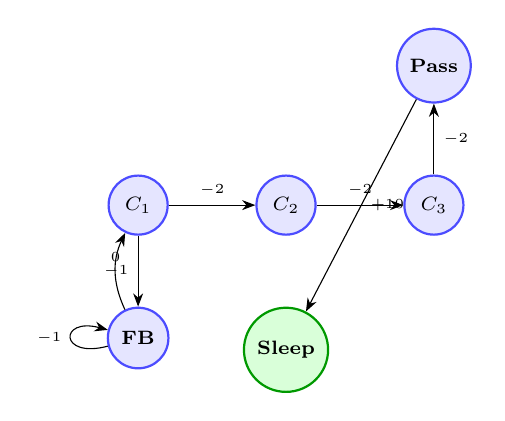
\begin{tikzpicture}[
        node distance=1.1cm,
        state/.style={circle,draw=blue!70,fill=blue!10,thick,
                      minimum size=0.75cm,font=\scriptsize\bfseries},
        term/.style={circle,draw=green!60!black,fill=green!15,thick,
                     minimum size=0.75cm,font=\scriptsize\bfseries},
        >=Stealth, font=\tiny
      ]
      \node[state] (C1) {$C_1$};
      \node[state] (C2) [right=of C1] {$C_2$};
      \node[state] (C3) [right=of C2] {$C_3$};
      \node[state] (Pass)[above=0.9cm of C3] {Pass};
      \node[state] (FB) [below=0.9cm of C1] {FB};
      \node[term]  (Slp)[below=0.9cm of C2] {Sleep};

      \draw[->] (C1) -- node[above]{$-2$} (C2);
      \draw[->] (C2) -- node[above]{$-2$} (C3);
      \draw[->] (C3) -- node[right]{$-2$} (Pass);
      \draw[->] (Pass)-- node[right]{$+10$}(Slp);
      \draw[->] (C1) -- node[left]{$-1$} (FB);
      \draw[->] (FB) to[loop left] node[left]{$-1$} (FB);
      \draw[->] (FB) to[bend left=25] node[above]{$0$} (C1);
    \end{tikzpicture}
  \end{columns}
\end{frame}

% ─────────────────────────────────────────────────────────────
\begin{frame}{Q1 -- Bellman Expectation: $\Vpi$ and $\Qpi$}
  \textbf{State-value function under policy $\pi$:}
  \[
    \boxed{\Vpi(s) = \sum_a \pi(a|s)\sum_{s'} P(s'|s,a)\bigl[R(s,a,s') + \gamma\,\Vpi(s')\bigr]}
  \]

  \textbf{Action-value (Q) function:}
  \[
    \boxed{\Qpi(s,a) = \sum_{s'} P(s'|s,a)\bigl[R(s,a,s') + \gamma\,\Vpi(s')\bigr]}
  \]

  \textbf{Consistency relation:}
  \[
    \Vpi(s) = \sum_a \pi(a|s)\,\Qpi(s,a)
  \]
\end{frame}

% ─────────────────────────────────────────────────────────────
\begin{frame}{Q1 -- Bellman Expectation: Iterative Evaluation}
  \begin{block}{Iterative Policy Evaluation}
    Start from $V_0 = \mathbf{0}$, repeat until $\|V_{k+1}-V_k\|_\infty < \theta$:
    \[
      V_{k+1}(s) = \sum_a \pi(a|s)\sum_{s'} P(s'|s,a)\bigl[R + \gamma\,V_k(s')\bigr]
    \]
  \end{block}

  \medskip
  \textbf{Linear system} (uniform policy, $\gamma=1$, $V(\text{Sleep})=0$):
  \small
  \begin{align*}
    V(C_1) &= \tfrac{1}{2}[-2+V(C_2)] + \tfrac{1}{2}[-1+V(\text{FB})]\\
    V(C_2) &= \tfrac{1}{2}[-2+V(C_3)] + \tfrac{1}{2}[-2+0]\\
    V(C_3) &= \tfrac{1}{3}[-2+V(\text{Pass})] + \tfrac{1}{3}[1+0.2\,V(C_1)+0.4\,V(C_2)+0.4\,V(C_3)]\\
    V(\text{FB}) &= \tfrac{1}{2}[-1+V(\text{FB})] + \tfrac{1}{2}[0+V(C_1)]
  \end{align*}
\end{frame}

% ─────────────────────────────────────────────────────────────
\begin{frame}{Q1 -- Computed Results: $V^\pi$, $V^*$, $\pi^*$}
  \begin{columns}[T]
    \column{0.48\textwidth}
    \begin{block}{$V^\pi$ vs $V^*$ ($\gamma=1$)}
      \scriptsize
      \begin{tabular}{lrr}
        \toprule
        State & $V^\pi$ (uniform) & $V^*$ \\
        \midrule
        $C_1$  & $-3.31$ & $6.00$ \\
        $C_2$  & $+0.69$ & $8.00$ \\
        $C_3$  & $+5.38$ & $10.00$ \\
        Pass   & $+10.00$ & $10.00$ \\
        FB     & $-4.31$ & $6.00$ \\
        Sleep  & $0.00$ & $0.00$ \\
        \bottomrule
      \end{tabular}
    \end{block}

    \column{0.48\textwidth}
    \begin{block}{Optimal Policy $\pistar$}
      \scriptsize
      \begin{tabular}{ll}
        \toprule
        State & $\pistar(s)$ \\
        \midrule
        $C_1$  & \textbf{Study} \\
        $C_2$  & \textbf{Study} \\
        $C_3$  & \textbf{Study} \\
        Pass   & \textbf{Sleep} \\
        FB     & \textbf{Quit} \\
        \bottomrule
      \end{tabular}

      \medskip
      \textbf{Bellman Optimality:}
      \[
        \Vstar(s) = \max_a \Qstar(s,a)
      \]
    \end{block}
  \end{columns}
\end{frame}

% ============================================================
\section{Q2: Iterative Policy Evaluation -- Grid World}
% ============================================================

\begin{frame}{Q2 -- Grid World Setup (Lecture 3, pp.~10--11)}
  \begin{columns}[T]
    \column{0.48\textwidth}
    \textbf{4$\times$4 grid world:}
    \begin{itemize}
      \item States $0\ldots15$; terminals: $\{0, 15\}$
      \item Uniform random policy: $\pi(a|s)=\tfrac{1}{4}$
      \item Actions: N, S, W, E (reflect at edges)
      \item $R=-1$ per step; $\gamma=1$ (undiscounted)
    \end{itemize}

    \medskip
    \textbf{One sweep:}
    \[
      V_{k+1}(s) = \frac{1}{4}\sum_{a}\bigl[R + V_k(s'(s,a))\bigr]
    \]

    \column{0.48\textwidth}
    \begin{center}
    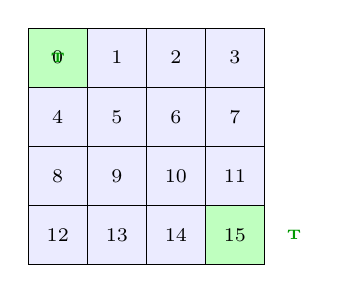
\begin{tikzpicture}[scale=0.75]
      \foreach \r in {0,...,3}{
        \foreach \c in {0,...,3}{
          \pgfmathtruncatemacro{\s}{\r*4+\c}
          \pgfmathtruncatemacro{\isT}{ifthenelse(\s==0 || \s==15,1,0)}
          \ifnum\isT=1
            \fill[green!25] (\c,-\r) rectangle ++(1,-1);
          \else
            \fill[blue!8] (\c,-\r) rectangle ++(1,-1);
          \fi
          \draw (\c,-\r) rectangle ++(1,-1);
          \node[font=\scriptsize] at (\c+0.5,-\r-0.5) {\s};
        }
      }
      \node[font=\tiny\bfseries,green!60!black] at (0.5,-0.5) {T};
      \node[font=\tiny\bfseries,green!60!black] at (4.5,-3.5) {T};
    \end{tikzpicture}
    \end{center}
  \end{columns}
\end{frame}

% ─────────────────────────────────────────────────────────────
\begin{frame}{Q2 -- Hand Computation: $k=1$ and $k=2$}
  \begin{columns}[T]
    \column{0.48\textwidth}
    \begin{block}{$k=1$: from $V_0=0$}
      All 4 actions give $R=-1$, $V_0(s')=0$:
      \[
        V_1(s) = \tfrac{1}{4}(-1\times 4) = -1.0
        \quad\forall s\notin\{0,15\}
      \]
    \end{block}

    \column{0.48\textwidth}
    \begin{block}{$k=2$: State 1 (top row, col~1)}
      \scriptsize
      N$\to$1 (wall): $-1+(-1)=-2$\\
      S$\to$5: $-1+(-1)=-2$\\
      W$\to$0 (term): $-1+0=-1$\\
      E$\to$2: $-1+(-1)=-2$\\[4pt]
      \[
        V_2(1) = \tfrac{1}{4}(-2-2-1-2) = \mathbf{-1.75}
      \]
      \[
        V_2(5) = \tfrac{1}{4}(-2\times4) = \mathbf{-2.00}
      \]
    \end{block}
  \end{columns}

  \medskip
  \begin{alertblock}{Key detail}
    N from row~0 \emph{reflects} back to same cell (wall), not wrapping to terminal~0.
  \end{alertblock}
\end{frame}

% ─────────────────────────────────────────────────────────────
\begin{frame}[fragile]{Q2 -- Hand Computation: $k=3$ and $k\to\infty$}
  \begin{columns}[T]
    \column{0.48\textwidth}
    \begin{block}{$k=3$: State 1}
      \scriptsize
      N$\to$1: $-1+(-1.75)=-2.75$\\
      S$\to$5: $-1+(-2.00)=-3.00$\\
      W$\to$0: $-1+0=-1.00$\\
      E$\to$2: $-1+(-2.00)=-3.00$\\[4pt]
      \[
        V_3(1) = \tfrac{1}{4}(-9.75) = \mathbf{-2.4375}
      \]

      \medskip\ttfamily\scriptsize
      \begin{semiverbatim}
V = iterative\_policy\_eval(k=3)
      \end{semiverbatim}
    \end{block}

    \column{0.48\textwidth}
    \begin{block}{$k\to\infty$: Convergence}
      \[
        V_k \xrightarrow{\|\cdot\|_\infty} V^\pi
      \]
      \scriptsize
      \begin{enumerate}
        \item Monotone decrease in $k$
        \item Convergence in ${\approx}200$ sweeps ($\theta{=}10^{-6}$)
        \item Cells near terminals $\approx 0$;\\
              corner~10 $\to\approx -14$
        \item Greedy policy from $V^\pi$:\\
              always toward nearest terminal
      \end{enumerate}
    \end{block}
  \end{columns}
\end{frame}

% ============================================================
\section{Q3: Jack's Car Rental}
% ============================================================

\begin{frame}{Q3 -- Jack's Car Rental: MDP (Lecture 3, pp.~14--15)}
  \begin{columns}[T]
    \column{0.50\textwidth}
    \textbf{Two locations; rent/return $\sim$ Poisson:}\\[4pt]

    \begin{tabular}{ll}
      \toprule
      Parameter & Value \\
      \midrule
      Max cars / loc & 20 \\
      Max moves / night & 5 \\
      Rental reward & $+\$10$ \\
      Move cost & $\$2$/car \\
      $\lambda_{\text{rent1}},\lambda_{\text{rent2}}$ & 3,\ 4 \\
      $\lambda_{\text{ret1}},\lambda_{\text{ret2}}$ & 3,\ 2 \\
      $\gamma$ & 0.9 \\
      \bottomrule
    \end{tabular}

    \column{0.46\textwidth}
    \begin{block}{State \& Action}
      $s=(n_1,n_2)$: cars at start of day\\
      $a\in[-5,5]$: move loc2$\to$loc1
    \end{block}

    \begin{block}{Bellman Equation}
      \scriptsize
      \[
        V(s) = {-2|a|}+\E\!\bigl[10\cdot r + \gamma V(s')\bigr]
      \]
    \end{block}

    \begin{alertblock}{Speed-up}
      \scriptsize
      Precompute $\text{EXP\_REW}[n]$, $\text{TRANS}[n,n']$\\
      $\Rightarrow$ matrix-vector product per state
    \end{alertblock}
  \end{columns}
\end{frame}

% ─────────────────────────────────────────────────────────────
\begin{frame}{Q3 -- Precomputed Dynamics \& Policy Iteration}
  \begin{columns}[T]
    \column{0.52\textwidth}
    \textbf{Precomputed (per location):}
    \[
      \text{EXP}[n] = \sum_{k=0}^{11} P(k;\lambda)\cdot\min(k,n)\cdot 10
    \]
    \[
      \text{TRANS}[n,n'] = \sum_{\text{req,ret}} P_r P_d\,\mathbf{1}[n'=\cdots]
    \]

    \textbf{Future value (matrix product):}
    \[
      \E[V(n_1',n_2')] = T_1[n_1,:]\cdot V\cdot T_2[n_2,:]^\top
    \]

    \column{0.44\textwidth}
    \begin{block}{Policy Iteration}
      \textbf{1.} Evaluate $V^{\pi_k}$\\
      \quad (Bellman until $\|\Delta V\|<\theta$)\\[4pt]
      \textbf{2.} Improve\\
      \quad $\pi_{k+1}(s)=\arg\max_a Q(s,a)$\\[4pt]
      \textbf{3.} Repeat until $\pi_{k+1}=\pi_k$\\[4pt]
      \textbf{Result:} converges in $\approx\!4$ steps
    \end{block}

    \begin{block}{Interpretation}
      \scriptsize
      Higher $\lambda_{\text{rent2}}=4$:\\
      move cars loc1$\to$loc2 when loc2 needs more.
    \end{block}
  \end{columns}
\end{frame}

% ============================================================
\section{Q4: Contraction Mapping Theorem}
% ============================================================

\begin{frame}{Q4 -- Setup: Banach Fixed-Point Theorem}
  \textbf{Finite MDP:} $(S,\mathcal{A},P,R,\gamma)$, $\gamma\in[0,1)$.

  \medskip
  Space of bounded value functions with sup-norm:
  \[
    \norm{V} = \max_{s\in S}|V(s)|
    \qquad (\mathcal{V},\|\cdot\|_\infty) \text{ is complete}
  \]

  \begin{theorem}[Banach Fixed-Point]
    If $T:\mathcal{V}\to\mathcal{V}$ satisfies
    $\norm{TV_1-TV_2}\leq\gamma\,\norm{V_1-V_2}$ for some $\gamma\in[0,1)$,\\
    then $T$ has a \textbf{unique fixed point} $V^*$ and
    \[
      \norm{T^k V_0 - V^*}\leq \gamma^k\,\norm{V_0-V^*}\to 0
    \]
  \end{theorem}
\end{frame}

% ─────────────────────────────────────────────────────────────
\begin{frame}{Q4 -- $\Tpi$ is a $\gamma$-Contraction}
  Define: $(\Tpi V)(s) = \sum_a\pi(a|s)\sum_{s'}P(s'|s,a)\bigl[R+\gamma V(s')\bigr]$

  \begin{proof}
    \vspace{-4pt}
    \begin{align*}
      |(\Tpi V_1)(s) - (\Tpi V_2)(s)|
      &= \gamma\Bigl|\sum_a\pi(a|s)\sum_{s'}P(s'|s,a)[V_1(s')-V_2(s')]\Bigr|\\
      &\leq \gamma\,\norm{V_1-V_2}\underbrace{\textstyle\sum_a\pi(a|s)\sum_{s'}P(s'|s,a)}_{=1}
    \end{align*}
    Take $\max_s$: $\;\norm{\Tpi V_1-\Tpi V_2}\leq\gamma\,\norm{V_1-V_2}$.\quad\qed
  \end{proof}

  \begin{alertblock}{Consequence}
    Iterative policy evaluation converges to the unique $V^\pi$ from \emph{any} $V_0$.
  \end{alertblock}
\end{frame}

% ─────────────────────────────────────────────────────────────
\begin{frame}{Q4 -- $\Tstar$ is a $\gamma$-Contraction}
  Define: $(\Tstar V)(s) = \max_a\sum_{s'}P(s'|s,a)\bigl[R+\gamma V(s')\bigr]$

  \begin{proof}
    Using $|\max f - \max g|\leq\max|f-g|$:
    \[
      |(\Tstar V_1)(s)-(\Tstar V_2)(s)|
      \leq \gamma\,\norm{V_1-V_2}
    \quad\Rightarrow\quad
      \norm{\Tstar V_1-\Tstar V_2}\leq\gamma\,\norm{V_1-V_2}\quad\qed
    \]
  \end{proof}

  \begin{columns}[T]
    \column{0.5\textwidth}
    \begin{block}{Value Iteration Bound}
      \[
        \norm{V_k-\Vstar}\leq\gamma^k\,\norm{V_0-\Vstar}
      \]
    \end{block}

    \column{0.46\textwidth}
    \begin{block}{Numerical Verification}
      \scriptsize
      For $\gamma\in\{0.5,0.9,0.99\}$, 500 random pairs:
      \[
        \frac{\norm{TV_1-TV_2}}{\norm{V_1-V_2}}\leq\gamma+10^{-9}\ \checkmark
      \]
    \end{block}
  \end{columns}
\end{frame}

% ─────────────────────────────────────────────────────────────
\begin{frame}{Q4 -- Policy Iteration Convergence}
  \begin{theorem}[Policy Iteration Convergence]
    Policy iteration converges to $\pistar$ in finitely many steps.
  \end{theorem}

  \begin{proof}[Sketch]
    \begin{enumerate}
      \item \textbf{Monotone improvement} (greedy step always $\geq$ current policy):
      \[
        V^{\pi'}(s)\geq Q^\pi(s,\pi'(s))=\max_a Q^\pi(s,a)\geq V^\pi(s)
      \]
      \item \textbf{Finite} policies: at most $|\mathcal{A}|^{|S|}$ deterministic policies.
      \item \textbf{Monotone~+~Finite $\Rightarrow$ terminates.}
        At termination $\pi^{k+1}=\pi^k$, so $V^{\pi^k}$ satisfies the Bellman\\
        Optimality Equation $\Rightarrow$ $V^{\pi^k}=V^*$.\qed
    \end{enumerate}
  \end{proof}
\end{frame}

% ─────────────────────────────────────────────────────────────
\begin{frame}{Q4 -- Convergence Rate ($\gamma=0.9$, Student MDP)}
  \begin{center}
  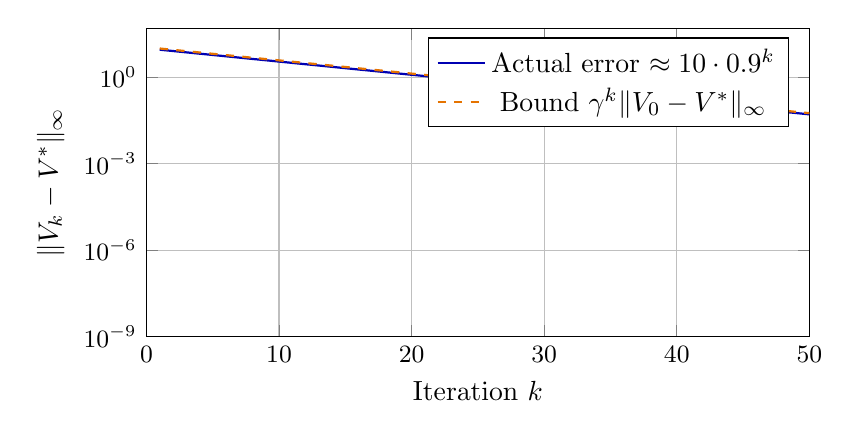
\begin{tikzpicture}
    \begin{semilogyaxis}[
      width=10cm, height=5.5cm,
      xlabel={Iteration $k$}, ylabel={$\|V_k-V^*\|_\infty$},
      legend pos=north east,
      grid=both, minor grid style={opacity=0.3},
      xmin=0, xmax=50, ymin=1e-9, ymax=50,
      tick label style={font=\small},
    ]
    \addplot[blue!70!black, thick, domain=1:50, samples=50]
      {10 * 0.9^x};
    \addlegendentry{Actual error $\approx 10\cdot 0.9^k$}
    \addplot[orange!90!black, thick, dashed, domain=1:50, samples=50]
      {10 * 0.9^x * 1.1};
    \addlegendentry{Bound $\gamma^k\|V_0-V^*\|_\infty$}
    \end{semilogyaxis}
  \end{tikzpicture}
  \end{center}
\end{frame}

% ============================================================
\section{Summary}
% ============================================================

\begin{frame}{Summary}
  \begin{center}
    \begin{tabular}{clll}
      \toprule
      \textbf{\#} & \textbf{Topic} & \textbf{Key Result} & \textbf{Method} \\
      \midrule
      Q1 & Student MDP &
        $V^\pi, Q^\pi, V^*, Q^*, \pi^*$ &
        Bellman + Value Iter. \\[4pt]
      Q2 & Grid World &
        $V_k$ exact for $k=1,2,3$; $V_k\to V^\pi$ &
        Iter. Policy Eval. \\[4pt]
      Q3 & Jack's Rental &
        Optimal policy in $\approx\!4$ PI steps &
        Policy Iteration \\[4pt]
      Q4 & Contraction &
        $\|\Tpi V_1-\Tpi V_2\|_\infty\leq\gamma\|V_1-V_2\|_\infty$ &
        Banach Theorem \\
      \bottomrule
    \end{tabular}
  \end{center}

  \bigskip
  \begin{block}{Unified message}
    $\Tpi$ and $\Tstar$ are $\gamma$-contractions $\Rightarrow$ iterative methods converge
    to unique fixed points $V^\pi$ and $V^*$. Policy iteration is monotone + finite
    $\Rightarrow$ converges to $\pistar$.
  \end{block}
\end{frame}

% ── References ───────────────────────────────────────────────
\begin{frame}{References}
  \begin{itemize}
    \item D.~Silver, \textit{Lecture 2: Markov Decision Processes}, UCL RL Course, 2015.
    \item D.~Silver, \textit{Lecture 3: Planning by Dynamic Programming}, UCL RL Course, 2015.
    \item R.~Sutton \& A.~Barto, \textit{Reinforcement Learning: An Introduction}, 2nd ed., MIT Press, 2018.
    \item S.~Banach, ``Sur les op{\'e}rations dans les ensembles abstraits,''
          \textit{Fundamenta Mathematicae}, 3:133--181, 1922.
  \end{itemize}

  \bigskip
  \begin{center}
    \LARGE\textbf{Thank you!}\\[6pt]
    \large\textbf{Group 4} $\;|\;$ Questions?
  \end{center}
\end{frame}

\end{document}
